
        The telescope system software runs on Linux servers and the basic understanding of the Linux operating system is required in order to operate the telescope. The Telescope Operator will also use Portal’s CAM graphical user interface referred to as GUI in order to interact with the telescope system. In order for anyone to interact with the telescope system, they need to have been given access via CAM portal.  The person needs a username and password to login into the system. When a person logs in for the first time on the system in order to control and monitor MeerKAT telescope system, the following is important to note. The system has many server nodes that are used for controlling and monitoring various parts of the system.  The most used servers nodes are:
        \begin{itemize}
\item{} \server{portal.mkat.karoo.kat.ac.za} and
\item{} \server{obs.mkat.karoo.kat.ac.za} 
\end{itemize}
The naming convention for the server nodes is always\\ $<$\server{server}$>$.$<$\server{telescope}$>.<$\server{site}$>$\server{.kat.ac.za.}, with :
\begin{itemize}
\item{} the first parameter is server node name
\item{} the second is the telescope (Currently: \server{mkat, kat7, mkat-rts}) and
\item{} the third is karoo for site systems different from lab systems.
\end{itemize}
\subsection{Portal Server}
The URL of where to find the GUI is \server{http://portal.mkat.karoo.kat.ac.za/}. 
The login details to the portal link above will be provided by CAM admistrator.
The landing page is as shown in \textbf{Figure}~\ref{fig:image71}. 
\clearpage
\begin{figure}[!thb]
	\centering
	%\includegraphicsdpi{100}{}{bur1.png}     
	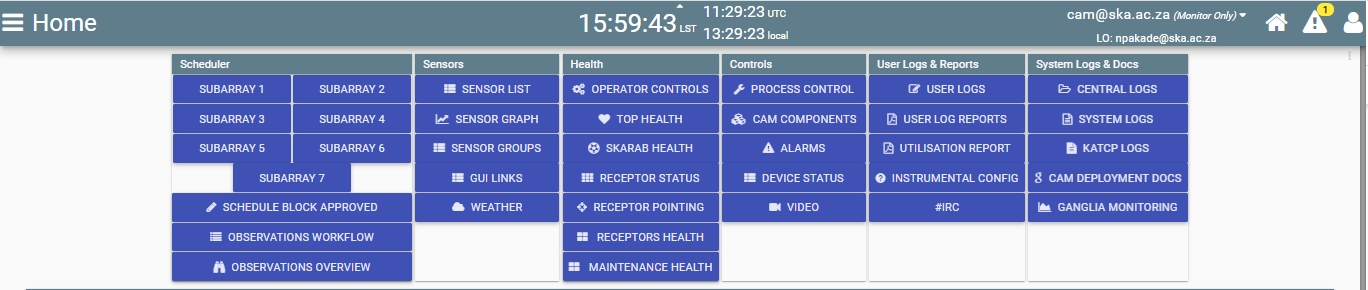
\includegraphics[scale=0.3]{Chapters/images/image71.png}
	
	%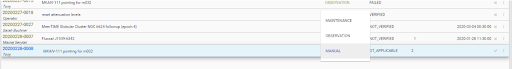
\includegraphics[resolution=100]{bur1.png}
	\caption{CAM GUI home page}
	\label{fig:image71}
\end{figure}




This will allow one to monitor the telescope system but will not be able to control the system. The person will have to be given the lead operator role (LO) or expert role in order to control the telescope for safety reasons. This page will allow one to access different functionality of the telescope system, monitoring and control i.e. if for instance one is interested in building and running subarray 1, the configuring of a subarray, one will click and open “SUBARRAY1 tab. This page will be shown as in \textbf{Figure}~\ref{fig:image38} below.

\begin{figure}[!thb]
	\centering
	%\includegraphicsdpi{100}{}{bur1.png}     
	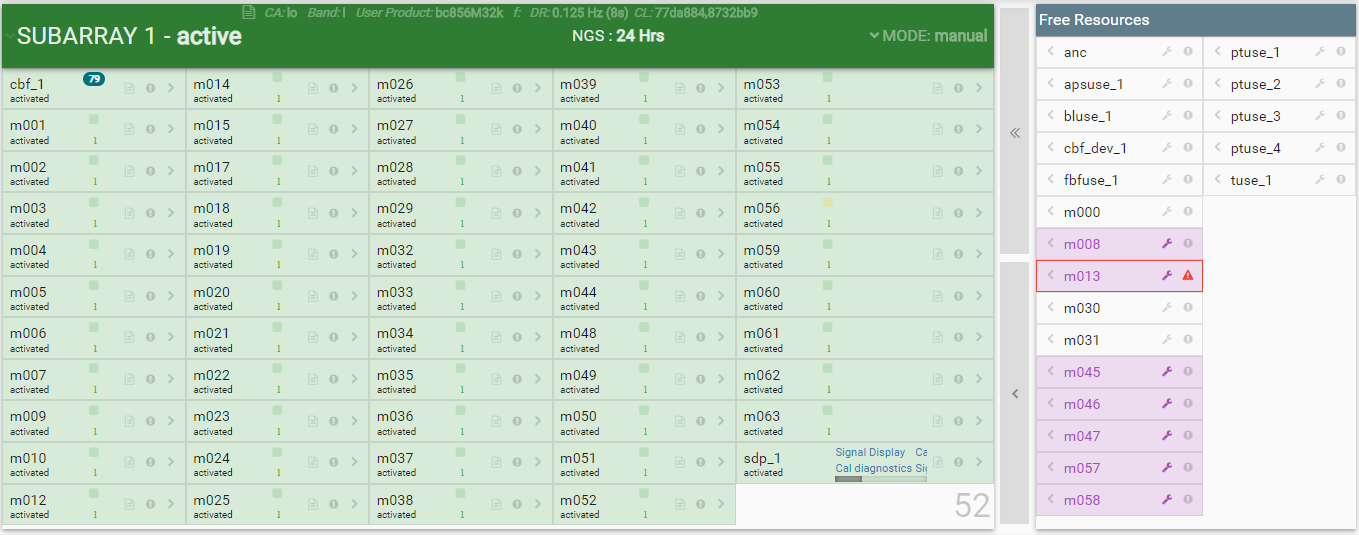
\includegraphics[scale=0.3]{Chapters/images/image38.png}
	
	%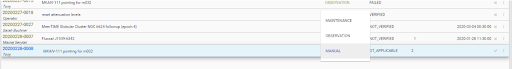
\includegraphics[resolution=100]{bur1.png}
	\caption{CAM GUI Subarray1 window}
	\label{fig:image38}
\end{figure}




In order to learn more about the GUI and the telescope system, the user must familiarise with different tabs on the GUI. More information will be discussed in the following sections of this document. 

\subsection{Obs Server/Machine}
The node server \server{“obs.mkat.karoo.kat.ac.za”} allows interaction with the live system via the command line and ipython interface. This is where the instructions to create a schedule block SB is provided.The user is required to command the telescope in the Linux environment from the command line using Linux and python commands. 
\clearpage
The user will be given credentials to login into the server. The server node to login using ssh command is \server{“obs.mkat.karoo.kat.ac.za” } and this will open up a page as shown in \textbf{Figure}~\ref{fig:image87}.

%\begin{figure}[!thb]
%	\centering
%	%\includegraphicsdpi{100}{}{bur1.png}     
%	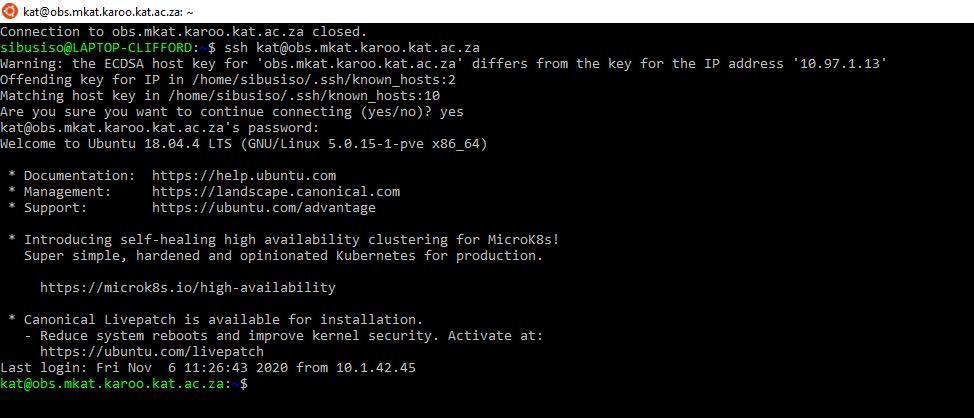
\includegraphics[scale=0.45]{Chapters/images/image87.png}
%	
%	%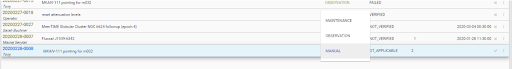
\includegraphics[resolution=100]{bur1.png}
%	\caption{Terminal ssh login to obs machine}
%	\label{fig:image87}
%\end{figure}
\begin{figure}[!thb]
	\centering
	%\includegraphicsdpi{100}{}{bur1.png}     
	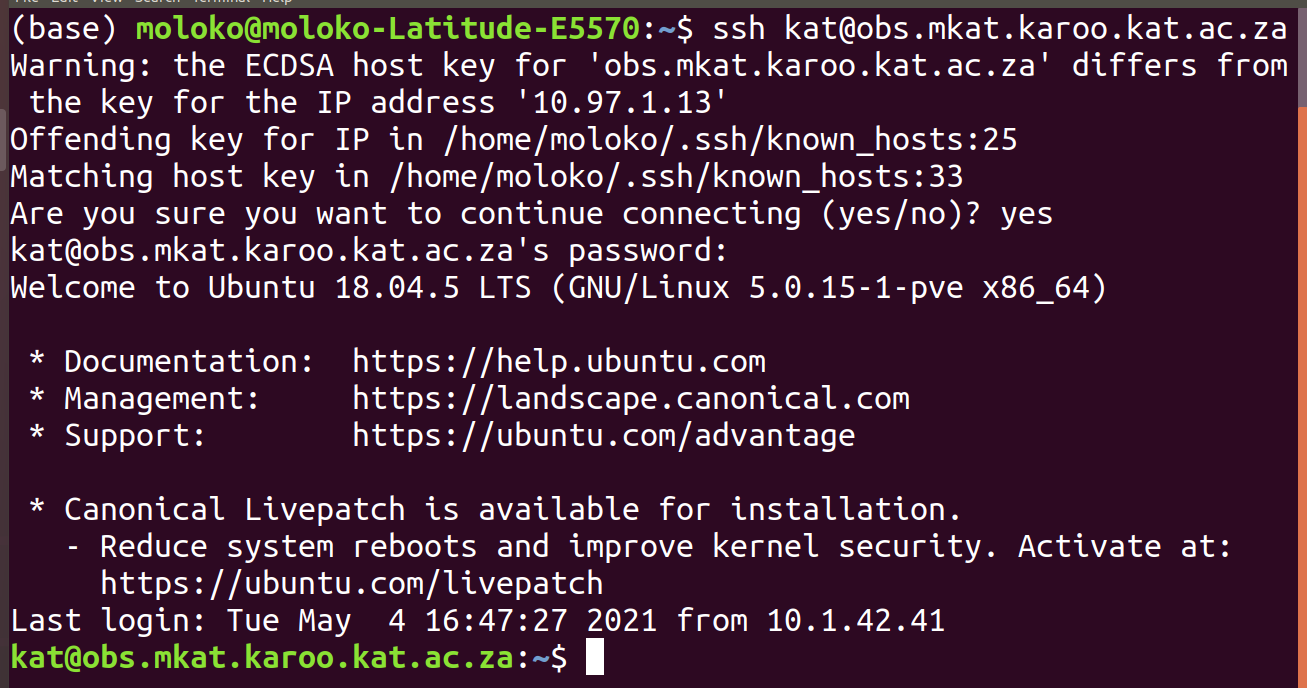
\includegraphics[scale=0.33]{Chapters/images/terminal.png}
	
	%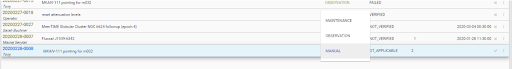
\includegraphics[resolution=100]{bur1.png}
	\caption{Terminal ssh login to obs machine}
	\label{fig:image87}
\end{figure}